\chapter{Introduction}\label{chapter:introduction}
\section{Structure of the Material}

Each chapter is designed to take 90-105 minutes of exercise time\footnote{This was the initial intention, but due to organizational reasons, some chapters may not have the appropriate amount of content now.}.
The "Examples" and easy "Exercises" with hints are mainly intended for beginners, and many of them can be solved in 5-10 minutes once understood. However, if you are tackling them for the first time, we recommend that you estimate about 5 times longer.
For experienced users, multiple exercises with different levels of difficulty are provided. The time required varies depending on the level of proficiency, but as a guideline, when a problem name has one $\star$ mark, the difficulty increases by about 5 times (for example, measured by the time required to create an answer). Also, some problems may assume knowledge from later chapters. Therefore, instead of solving all the problems in each chapter before moving on to the next, we recommend that you move on to the next chapter once you have solved the easy problems without a mark. Once you have gone through the examples and seen what topics are covered, you will likely find that you can solve more problems in the second round. Furthermore, problems with two or more $\star$ marks may have some relation to the content of the chapter, but may not be directly related to the solution method. This is because determining which strategy is effective is one of the interesting aspects of learning problem-solving.

\paragraph{Legend}
Links within the material are shown in dark green (e.g., Chapter \ref{chapter:introduction}, Reference \cite{book:pcc}).
Also, external links are shown in blue (e.g., \url{http://www.graco.c.u-tokyo.ac.jp/icpc-challenge/}).

\paragraph{Supplementary Note for Students (Planning to) Take Practical Programming in the First Semester of the College of Arts and Sciences}
The seminars that will be held from now on do *not* assume that you have studied this material in advance. In other words, materials for beginners will continue to be provided alongside exercises for experienced users. The themes covered will overlap with this material in some parts and not in others.
\section{Programming Languages}

The following languages are considered for learning:
\begin{itemize}
\item \textbf{C++} (Recommended: This is the main target language)
\item Java
\item \textbf{Python3} (Recommended: However, some problems may not be solvable due to time limits)
\item Ruby (Some problems may not be solvable due to time limits)
\end{itemize}

Learning with the following languages is not recommended:
\begin{itemize}
\item C (Reason: Due to the limited standard library. For example, it lacks associative array functionality.)\\
  C language users should use C++. The functionality required for the exercises in this material is only a small part of the whole C++, so you can borrow only that part and write the rest as if it were C. In other words, it should be less difficult than generally relearning C++.
\item Python2 (Reason: There are various pitfalls such as variable scope and character encoding)
\end{itemize}
\section{Textbooks and References}

It is assumed that the reader of this material is able to write short code involving loops and conditional branches as intended, and has also learned about recursion.
Therefore, if you are truly encountering programming for the first time, it is recommended that you first learn from another book. If you already have a purchased book, that is sufficient, but if you are purchasing a new one, "Introduction to C/C++ Programming Starting with Online Judge" \cite{book:aojcpp} has a good connection with this material in that it uses AOJ.

In the text, we may refer to
\pccbook{} as "Algorithm and Data Structures for Competitive Programming" and
\pcaojbook{} as "Programming Contest Challenge Book, Second Edition" (it goes without saying that these are masterpieces in this field).
Also, for those who have plenty of study time (and budget), we recommend taking the time to read up to Chapter 6 of "Algorithm Design" \cite{book:algorithmdesign}. Although it has many pages, it is written carefully, so it seems suitable for beginners among similar books (however, the author read the English version, so the evaluation of the Japanese version is an estimate). If you want to learn more deeply, "Introduction to Algorithms" \cite{book:algorithmintroduction} is also worth spending time studying.
\section{Online Judge Systems}

The problems in this material are taken from the following online judges. When creating the material, the person in charge checked the terms of use of each online judge to the extent possible, and judged that there would be no problem in referring to each problem in this material. However, please contact us if you notice anything.

\begin{itemize}
    \item Aizu Online Judge (\index{AOJ}) \url{http://judge.u-aizu.ac.jp}
    \item Peking University Judge Online for ACM/ICPC (\index{POJ}) \url{http://poj.org}
    \item Codeforces \url{http://www.codeforces.com/}
    \item szkopul \url{https://szkopul.edu.pl} (formerly \url{http://main.edu.pl/en})
\end{itemize}

When describing the sources, those from the domestic \index{ACM-ICPC} (\url{https://icpc.iisf.or.jp/}) and the ACM-ICPC Alumni Association (JAG; \url{http://acm-icpc.aitea.net/}) are simplified as much as possible within the range that they can be distinguished. For example, \jindex{国内予選}{kokunai yosen} refers to the Japanese ACM-ICPC, and the mock domestic preliminary refers to the regular practice session organized by the ACM-ICPC Alumni Association.
\section{Aizu Online Judge (AOJ)}

\subsection*{Creating an Account}

If you are a first-time user, you will need to create an account on \eindex{AOJ}. All systems can be used free of charge.
Please remember that each online judge is provided as a courtesy by its operators, so please use it in a way that \emph{does not cause any trouble}. In particular, \emphasizedunderline{do not forget your password}.

\paragraph{Creating an AOJ Account (First Time Only)}
Create an account from the Register/Setting link in the upper right corner of the page.
Remember your User ID and Password (save it in your browser or in an encrypted
file). Note that this communication is not https.
For Affiliation, enter something like the University of Tokyo. You do not need to fill in E-mail or URL.

Here, you can choose whether to make your submitted programs public or not. If you make them public (select ``public''), it may be convenient when asking for help with errors in your program. On the other hand, if you are trying to "test the behavior of other people's code snippets," copyright issues may arise, so it is better to keep them private (select ``private'').

\paragraph{Submitting to AOJ (Every Time)}

After logging in, with the problem statement displayed, click the icon with an upward arrow in a rectangle to display the form.


\includegraphics{aoj.eps}

If the ``Status'' of the row corresponding to your submission (see ``Author'') is ``\eindex{Accepted}'', then your answer is correct.

\paragraph{When the Answer is Not Correct}

There can be various reasons, so first, read the explanations to see which of the judge's responses applies and whether you have misunderstood how to use the system.
There are materials such as Terms of use
(\url{https://onlinejudge.u-aizu.ac.jp/#/term_of_use}),
Judge's replies (\url{https://onlinejudge.u-aizu.ac.jp/#/judges_replies}),
and a tutorial (\url{http://judge.u-aizu.ac.jp/onlinejudge/AOJ_tutorial.pdf}).

In general, \textbf{it is common for programs not to work as intended, even for experienced programmers!}.
Even if the program you have built does not work, it does not mean that everything is wrong. In many cases, it can be solved with a few small changes. Therefore, it is effective to check the operation of each part to see up to which point it is working correctly.
Programming on a computer has the advantage that \textbf{you can copy and undo}, so (unlike cooking, where you might be disappointed by wasting ingredients), do not be afraid to try various things.

There is also some know-how on how to recover from difficult situations (Appendix \ref{chapter:debug}), so it will be useful to gradually acquire it.
On the other hand, at an early stage of experience, we recommend that you \emphasizedunderline{do not spend more than 15 minutes worrying}.
Spending time worrying without a clue is not only painful, but also not very effective for learning at an early stage. It is better to rely on an instructor, senior, or friend, or to put it on hold and work on other problems to gain experience.
When consulting, it will be quicker to solve the problem if you verbalize it by specifying "it should work like this (the reason is this), but it actually works like that".
Note that the amount of time you can spend worrying meaningfully will increase as you become more proficient, such as 2 hours or 2 days.
\section{Input/Output and Problem Correspondence}

Let's try submitting a solution to a problem on AOJ.

\begin{psbox}{Rectangle}{AOJ}
Create a program to calculate the area and perimeter of a rectangle with a width of $a$ cm and a height of $b$ cm.
  \aojid{ITP1_1_C}
\end{psbox}

Follow these steps:
\begin{enumerate}
\item Understand the problem.
\item Consider the calculation procedure (in this case, understand that you need to calculate $a*b$ and $2*(a+b)$).
\item Write the program. Edit it with your preferred \index{editor}(Emacs, mi, etc.) and save it to a file.
\item Check the operation on your computer (required).
\item Submit to AOJ and confirm.
\end{enumerate}

\paragraph{Example Solutions}: Below are example solutions in each language and how to check the operation for the case of \texttt{a=3} and \texttt{b=5}.

\begin{pybox}
a,b = map(int, input().split())
area = a*b
perimeter = 2*(a+b)
print(area, perimeter)
\end{pybox}

\texttt{input()} reads a line, \texttt{split()} splits it by spaces\footnote{At this time, the trailing newline character and (if any) leading or consecutive spaces are also removed.}, and \texttt{map(int, ...)} converts each split element to an integer.

After saving the above content as \texttt{rectangle.py}, execute it on the \index{terminal}. \texttt{\$} is an abbreviation for the prompt and does not need to be entered by yourself (that is, type after \texttt{python3})\footnote{See HWB15.2 for details \url{https://hwb.ecc.u-tokyo.ac.jp/wp/information-2/cui/terminal/}}. Also, \texttt{\#} and the part to its right are supplementary explanations and do not need to be entered. Press the Enter key at the end of each line of input. Below, italics indicate input from the keyboard.

\begin{terminal}
$ python3 rectangle.py
3 5 # Input from the keyboard
15 16 # Program output display
\end{terminal}

\begin{cbox}
#include <iostream>
using namespace std;
int main() {
  int a,b;
  cin >> a >> b;
  int area = a*b;
  int perimeter = 2*(a+b);
  cout << area << ' ' << perimeter << "\n";
}
\end{cbox}

Save the above program as \texttt{rectangle.cc}, etc. Then compile and execute it.

An example of operation on the "Terminal" (in the case of MacOSX) is as follows:
\begin{terminal}[emph={Wall,fsanitize}]
$ g++ -std=c++11 -Wall -fsanitize=undefined rectangle.cc # Compile
$ ./a.out # Execute
3 5 # Input from the keyboard
15 16 # Program output display
\end{terminal}

\texttt{\#} and everything to its right are comments and do not need to be entered.
\eindex{-std=c++11} is a \index{compiler option} that enables the C++11 standard.
\eindex{-Wall} is an option that enables various warnings, and it is desirable to resolve any warning messages that appear. In particular, \emphasizedunderline{if there is a question about the program's operation}, \emphasizedunderline{resolve any prominent warnings before asking a question}. If you get a message that you don't know how to read, consult with someone.
\eindex{-fsanitize=undefined} enables a mechanism to catch runtime errors. It is desirable to keep it on during operation checks. See Chapter \ref{section:cpp-sanitize} for details.

\begin{warningbox}{C Language Prohibited}
  When reading this material, C language is insufficient, and it is necessary to use some of the functions of C++. We will introduce the necessary parts little by little, so get used to \texttt{iostream,cin,cout} etc. at this point.
\end{warningbox}
	
\begin{warningbox}{Prohibition of Programming on the Browser}
  You may be able to code simple problems on the browser, but this is not the case for the complex problems we will be dealing with in the future. Prepare an environment where you can compile and run on your PC with various data at this point.
\end{warningbox}

\begin{cbox}
#include <cstdio>
int main() {
  int a,b;
  scanf("%d %d", &a, &b);
  int area = a*b;
  int perimeter = 2*(a+b);
  printf("%d %d\n", area, perimeter);
}
\end{cbox}
In this material, we recommend that C language users migrate to C++, but even when using C++, you can use C's \texttt{scanf} and \texttt{printf} for input and output.

\begin{rbox}
a,b = gets.split(" ").map(&:to_i)
area = a*b
perimeter = 2*(a+b)
print sprintf("%d %d", area, perimeter)
\end{rbox}

After saving the above content as \texttt{rectangle.rb}, etc., execute it on the terminal.
\begin{terminal}
$ ruby rectangle.rb
\textit{3 5} # Input from the keyboard
15 16 # Program output
\end{terminal}

In the case of Java, due to the restrictions of the online judge system, it is always necessary to write the answer in a class called \texttt{Main}. For that purpose, it is necessary to save it with the file name \texttt{Main.java}, so create a folder for each problem and work there.
\begin{javabox}[emph={Main}]
import java.util.Scanner;
public class Main {
    public static void main(String[] args) {
	Scanner scanner = new Scanner(System.in);
	int a = scanner.nextInt(), b = scanner.nextInt();
	int area = a*b;
	int perimeter = 2*(a+b);
	System.out.println(area+" "+perimeter);
    }
}
\end{javabox}

\begin{terminal}
$ javac Main.java
$ java Main
\textit{3 5} # Input from the keyboard
15 16 # Program output display
\end{terminal}
\section{Practical Notes}\label{section:commands}
\subsection{Saving Folders}
In each chapter, we will handle multiple code snippets for samples and functionality verification.
Therefore, to avoid confusion, it is good practice to create a \index{folder} and save files with different names for each theme. And keep each of them working.
On the other hand, we do not recommend adding to a file you have already created, making it one huge file. If you do that, it will be difficult to compare the results of running two different codes later.

Here is an example of how to use the "Terminal" (in the case of MacOSX):
\begin{terminal}
$ mkdir programming
# (Create a folder, only the first time)
$ mkdir programming/chapter1
# (Do this for each chapter)
$ cd programming/chapter1
# (Change the current directory. Save the source code under \$HOME/programming/chapter1/)
\end{terminal}

\subsection{Testing with Files Using Standard Input/Output and Redirection}

This section introduces \textit{how to read data as long as it exists} and \textit{how to test using files}.
It is not necessary to master the contents of this section immediately, but it is desirable to learn them in the process of working on Chapters 2 and 3.

When dealing with large inputs and outputs, it is not appropriate to enter them manually from the keyboard.
(Manual input carries the risk of typos. Copying and pasting improves this somewhat, but there are limits to the amount of data, and there is still room for errors in selection. When verifying the correctness of a program, it is desirable to eliminate other uncertain factors 100\% and focus on the program itself.)

Each problem handles standard input and output, and the correctness of the program is determined by the output for the input. In many cases, the input is read and processed as long as there is input data.
So, let's start with an example. The following environment is basically assumed to be MacOSX, but it should also work on Ubuntu, Cygwin, etc.

\begin{itembox}[l]{Example Problem}
Create a program that reads a year, determines if it is a leap year, and outputs the number of days.
\end{itembox}

(Rough) Example program (C++): leap.cc

%\begin{codebox}
%// Is it every 4 years?
%#include <iostream>
%using namespace std;
%int main() {
%    int year;
%    while (cin >> year) { // cin is automatically converted to bool, so loop as long as input can be read
%      if (year % 4 == 0)
%        cout << 366 << endl;
%      else
%        cout << 365 << endl;
%    }
%}
%\end{codebox}
%
%\paragraph{Compilation}
%
%(As mentioned above, the \$ symbol indicates a command input to the terminal)
%
%In the case of C++:
%\begin{terminal}
%$ g++ -Wall leap.cc
%\end{terminal}
%
%In the case of Java:
%\begin{terminal}
%$ javac Main.java
%\end{terminal}

%\paragraph{Execution Example}
%Italics indicate input from the keyboard. To terminate, press Ctrl and type c or d. This operation is denoted as \^{}C or \^{}D.
%
%\begin{terminal}
%$ ./a.out
%\textit{2004}
%366
%\textit{1999}
%365
%\textit{1900}
%366
%\textit{2000}
%366
%\^{}D
%\end{terminal}
%
%\paragraph{Testing with Files}
%Typing on the keyboard every time you run the program is cumbersome, so we want to automate it.
%Therefore, we will explain testing using redirection and files.
%It is desirable to learn this at an early stage.
%
%Create correct input and output examples with an editor, and check the contents with the \texttt{cat} command:
%\begin{terminal}
%$ cat years.input
%2004
%1999
%1900
%2000
%$ cat years.output
%366
%365
%365
%366
%\end{terminal}
%
%Execution using \index{redirection} (reading from a file instead of keyboard input):
%\begin{terminal}
%$ ./a.out < years.input
%366
%365
%366
%366
%\end{terminal}
%
%Saving the execution result to a file (writing to a file instead of displaying it on the screen):
%\begin{terminal}
%$ ./a.out < years.input > test-output
%$ cat test-output
%366
%365
%366
%366
%\end{terminal}
%
%Automatic comparison using \index{diff}:
%\begin{terminal}
%$ diff -u test-output years.output
%--- years.output        Fri Oct 14 10:53:52 2005
%+++ test-output Fri Oct 14 10:53:56 2005
%@@ -1,4 +1,4 @@
% 366
% 365
%-365
%+366
% 366
%\end{terminal}
%It tells us that the 4th line is different.
%
%\begin{itembox}[l]{References:}
%\begin{itemize}
%\item HWB 15 Commands\\
%  \url{http://hwb.ecc.u-tokyo.ac.jp/wp/information-2/cui/}
%\item HWB 14.4 File Operations Using Commands\\
% \url{http://hwb.ecc.u-tokyo.ac.jp/wp/information-2/filesystem/cui-fs/}
%\end{itemize}
%\end{itembox}
%
%\subsection{Downloading Judge Data and Running it Locally}\label{run-judge-data}
%When you submit a program, it may result in \index{Wrong Answer}, \index{Time Limit Exceeded}, or \index{Runtime Error} instead of Accepted.
%
%Suppose you are solving a problem called \texttt{ITP1\_4\_D} and you get a Wrong Answer.
%
%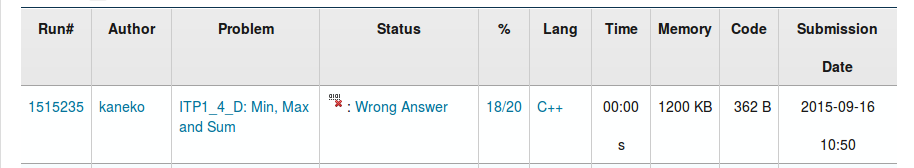
\includegraphics[width=.9\linewidth]{2.png}
%
%The number 18/20 near the center means that you answered correctly up to the 18th test case and failed on the 19th. You can click on that part, which is a hyperlink, to see the details.
%
%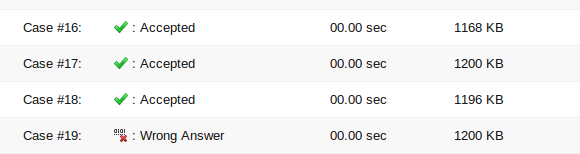
\includegraphics[width=.7\linewidth]{3.png}
%
%Furthermore, if you click on the line \texttt{Case \#19:}, you can see the actual data (depending on the problem).
%
%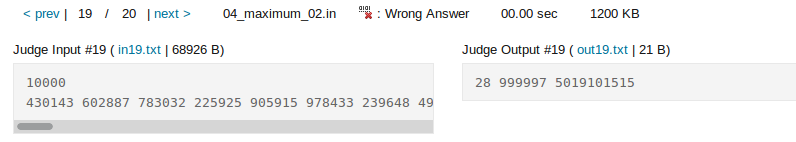
\includegraphics[width=.9\linewidth]{4.png}
%
%Let's try this data locally.
%Since the data is too large to copy and paste, first click on the \texttt{in19.txt} part to download it.
%Depending on your environment and browser, it will be saved in your download folder with a name like \texttt{ITP1\_4\_D\_in19.txt}. Execute it by redirection as appropriate.
%
%\begin{terminal}
%$ ./a.out < ~/Downloads/ITP1_4_D_in19.txt 
%28 999997 724134219  
%\end{terminal}
%
%Also, this time it is obvious at a glance that there is a difference between the program's output and the Judge Output, but in general, it is difficult to compare numbers with many digits like 5019101515 by eye (you may not notice even if one character is different), so it is better to download it and compare it with the \texttt{diff} command.
%
%Save the execution result to a file (write to a file instead of displaying it on the screen):
%\begin{terminal}
%$ ./a.out < sample-input.txt > my-output.txt
%$ cat my-output.txt
%1 17 37
%\end{terminal}
%
%Compare the two files:
%\begin{terminal}
%$ diff -u sample-output.txt my-output.txt
%\end{terminal}
%(Output will only be displayed if there are differences)